\section{Certified Lifting}\label{sec:method}
\begin{figure*}[t]\centering
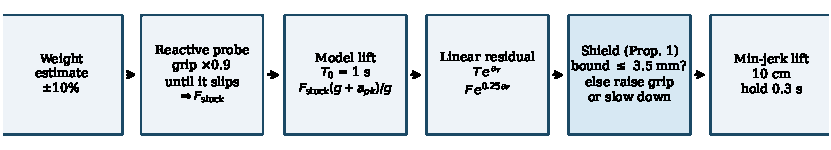
\includegraphics[width=\textwidth]{fig_method.pdf}
\caption{\textbf{Episode pipeline.} A wrist weight estimate and a reactive probe give the breakaway grip $\Fs$; the friction-model
controller proposes a lift; the residual policy rescales its duration and grip; the shield evaluates Proposition~\ref{prop:lift}
and, if the slip bound exceeds 3.5\,mm, raises the grip (grip axis) or lengthens the lift (time axis) until it does not,
declining if neither suffices. Then the gripper lifts the object 10\,cm along a minimum-jerk profile and holds for 0.3\,s.}\label{fig:method}
\end{figure*}

\subsection{Task}
A parallel gripper holds a rod of unknown mass $m\sim U[0.05,0.2]$\,kg and unknown static friction $\mu_s\sim U[0.4,0.8]$
at its centre of mass, with gravity along the rod axis. Kinetic friction is $\mu_k=\mu_s/r$, with the ratio $r\ge1$ also
unknown. The gripper lifts the rod by $H=10$\,cm along a minimum-jerk trajectory of duration $T$~\cite{flash1985},
\begin{equation}
z(t)=H\,(10s^3-15s^4+6s^5),\quad s=t/T,\qquad a_{pk}=\tfrac{10}{\sqrt3}\,\tfrac{H}{T^2}\approx5.77\,\tfrac{H}{T^2},
\end{equation}
at a constant grip $F$ per pad, then holds still for 0.3\,s. The rod is supported only by friction. Two pads with Coulomb
friction hold it while
\begin{equation}\label{eq:stick}
m\,(g+a(t))\;\le\;2\mu_s F,
\end{equation}
and once it slides its acceleration relative to the fingers is $g+a(t)-2\mu_kF/m$. A lift \emph{fails} if the rod slips
more than $S_{\rm tol}=5$\,mm relative to the fingers during the lift and hold, or is dropped. We want short lifts and low
grips without failures.

\subsection{Probing the breakaway grip}
Before lifting, the gripper estimates the breakaway grip with the palm still. The grip starts at $\hat m g/(2\cdot0.3)$, the
grip that would hold the estimated weight at $\mu=0.3$, and is multiplied by 0.9 every 0.4\,s (0.1\,s ramp, 0.3\,s hold)
while a slip monitor with 0.5\,mm noise watches. When the monitor reads more than 2.5\,mm since the step began, the grip
snaps to 2.5 times the grip that moved within 20\,ms, so the probe never lets the rod run away. The weight estimate
$\hat m$ is within $\pm10$\% of $m$ (wrist force sensing). The probe returns $\Fs$, the last grip at which the rod did not
move. Since the rod held at $\Fs$, \eqref{eq:stick} with $a=0$ gives $2\mu_s\Fs\ge mg$: $\Fs$ is an \emph{upper} bound on the
true breakaway grip $F_b=mg/(2\mu_s)$, and its step size makes it at most about 11\% above it.

\subsection{The friction-model controller}
The quasi-static Coulomb lift uses a fixed duration $T_0=1$\,s and the grip that just holds at peak acceleration if
$r=1$:
\begin{equation}
F_{\rm model}(T)=\Fs\,\frac{g+a_{pk}(T)}{g}.
\end{equation}
It is slow and, because $\Fs\ge F_b$, it carries a margin of up to 11\%.

\subsection{A slip bound for lifting}
\begin{proposition}[Lift slip bound]\label{prop:lift}
Let the palm follow an acceleration profile $a(t)$ from rest at constant grip $F$, let $\Fs$ be a grip at which the object
was observed stuck with the palm at rest, and let $r\le r_{\max}$. Then slip cannot begin while $g+a(t)\le gF/\Fs$.
Let $t_0$ be the first instant with $g+a(t_0)>gF/\Fs$ and define
\begin{equation}
\bar a(t)=g+a(t)-\frac{gF}{r_{\max}\Fs},\qquad \dot{\bar v}=\bar a\ \text{with}\ \bar v\ge0\ \text{(clipped)},\ \bar v(t_0)=0.
\end{equation}
Then the slip of the object relative to the fingers is at most $\bar s=\int_{t_0}\bar v\,dt$.
\end{proposition}
\noindent\textit{Proof sketch} (full proof in Appendix~\ref{app:proof}). Because the object held at $\Fs$, the static
capacity per unit mass at grip $F$ is $2\mu_sF/m=gF/F_b\ge gF/\Fs$, so \eqref{eq:stick} holds while $g+a\le gF/\Fs$.
While sliding, the kinetic capacity is $2\mu_kF/m=gF/(rF_b)\ge gF/(r_{\max}\Fs)$, so the relative acceleration is at most
$\bar a$; re-sticking can only lower it. A comparison argument gives $v(t)\le\bar v(t)$ and hence the bound.\hfill$\square$

The bound needs no knowledge of $m$, $\mu_s$ or $r$ beyond $\Fs$ and $r_{\max}$. We evaluate it over the whole commanded
profile: the 0.6\,s grip ramp and settle (during which the grip is at least $F$), the lift, and the 0.3\,s hold.
Figure~\ref{fig:bound} shows how it behaves.

\begin{figure*}[t]\centering
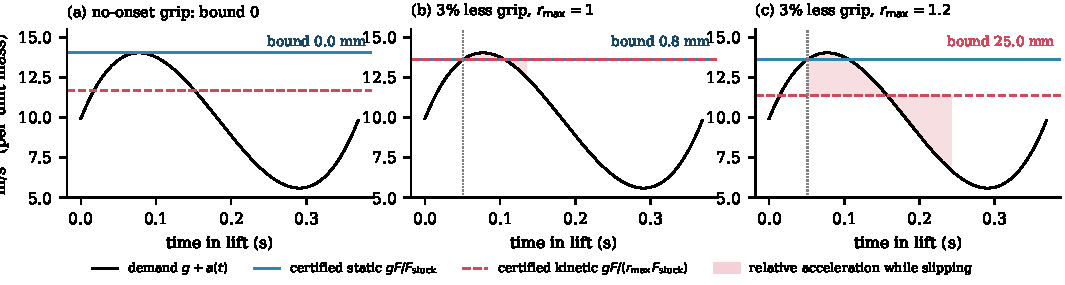
\includegraphics[width=\textwidth]{fig_bound.pdf}
\caption{\textbf{How Proposition~\ref{prop:lift} works} (minimum-jerk lift, $T=0.37$\,s). (a) At the no-onset grip
$F_{\rm model}(T)$ the demand never exceeds the certified static capacity and the bound is zero. (b) With 3\% less grip,
slip may begin near peak acceleration; if friction does not drop ($r_{\max}=1$) the excess is small and short, and the bound
is 0.8\,mm. (c) The same grip with a possible 20\% drop: from the moment slip may begin, the certified kinetic capacity is
far below the demand for most of the acceleration phase, and the bound jumps to 23\,mm. This cliff is why slip allowances
buy little (Section~\ref{sec:q4}).}\label{fig:bound}
\end{figure*}

\subsection{The shield}
A command $(T,F)$ is \emph{certified} if $\bar s\le s_{\lim}=S_{\rm tol}-1.5$\,mm, where 1.5\,mm is a sensing margin (three
standard deviations of the slip monitor). The \emph{grip projection} raises $F$ to the smallest certified grip (bisection,
up to 30\,N); the \emph{time projection} lengthens $T$ to the shortest certified duration (up to 2\,s). If neither exists,
the shield \emph{declines} and the lift falls back to the model controller's command. The shield uses $r_{\max}=1.2$
unless stated. It costs one bisection over a one-dimensional integral, under a millisecond in our implementation.

\subsection{The residual policy}
A linear policy maps six features of the probe to two actions through $\tanh$: the log ratio of $\Fs$ to the estimated
weight, the log ratio of the grip that moved to $\Fs$ (the probe's resolution), the estimated mass, the probe count, the
grip scale and a bias. The actions rescale the model's command,
\begin{equation}
T=T_0\,e^{a_T}\in[0.25,2]\,\mathrm{s},\qquad F=F_{\rm model}(T)\,e^{0.25\,a_F},\qquad a_T,a_F\in[-1,1],
\end{equation}
so zero weights reproduce the model controller and the grip action is relative to the model's grip \emph{for the chosen
duration}. The training reward is $-10$ for a failed lift and otherwise $-T/T_0-\lambda F/(10\,mg)$ with $\lambda=1$: one
second of lift time is worth ten object-weights of grip. Training uses antithetic evolution strategies with rank-based
fitness shaping~\cite{salimans2017,mania2018} and Adam~\cite{kingma2015} (Appendix~\ref{app:train}).

\begin{remark}[Why the residual can beat the model]
$F_{\rm model}$ is quasi-static and uses $\Fs\ge F_b$. Both make it conservative: Table~\ref{tab:val} shows that the grip
needed during a fast lift is 2--11\% below the quasi-static prediction, and $\Fs$ adds up to 11\%. A residual can find this
margin. It cannot know whether friction will drop once it uses it.
\end{remark}
